\documentclass[./../main.tex]{subfiles}
\graphicspath{{img/}}

\begin{document}
    \section{}
    
    Considera el campo escalar definido por:

    \begin{equation*}
        \phi(x, y) = x^{2} - y^{2}
    \end{equation*}

    en el dominio \(0 \leq x \leq L_{x}\), \(0 \leq y \leq L_{y}\).

    Determinar:

    \begin{enumerate}[label=\arabic*)]
        \item el gradiente del campo escalar,
        
        Calculamos el gradiente del campo escalar como

        \begin{align}
            \grad{{\phi(x, y)}} &= \Bigl( \pdv{\phi}{x}, \pdv{\phi}{y}, 0\Bigr),\nonumber\\
            \Aboxedmain{
                \grad{{\phi(x, y)}} &= (2x, -2y, 0).
                \label{eq:gradient-scalar-field}
            }
        \end{align}
        
        \item el Laplaciano del campo escalar,
        
        Recordemos que el Laplaciano de un campo escalar se define como

        \begin{equation*}
            \lap{\phi} = \dvg{(\grad{\phi})},
        \end{equation*}

        entonces simplemente calculamos la divergencia de \cref{eq:gradient-scalar-field}:

        \begin{align*}
            \lap{{\phi(x, y)}} &= \pdv{(2x)}{x} - \pdv{(2y)}{y},\\
            &= 2 - 2,\\
            \Aboxedmain{
                \lap{{\phi(x, y)}} &= 0.
            }
        \end{align*}
    \end{enumerate}

    \pagebreak
    Graficar:
    \begin{enumerate}[label=\arabic*), resume]
        \item el campo escalar \(\phi\),
        
        La gráfica del campo escalar \(\phi(x, y) = x^{2} - y^{2}\) se muestra en la \cref{fig:scalar-field}.

        \begin{figure}[htb]
            \centering
            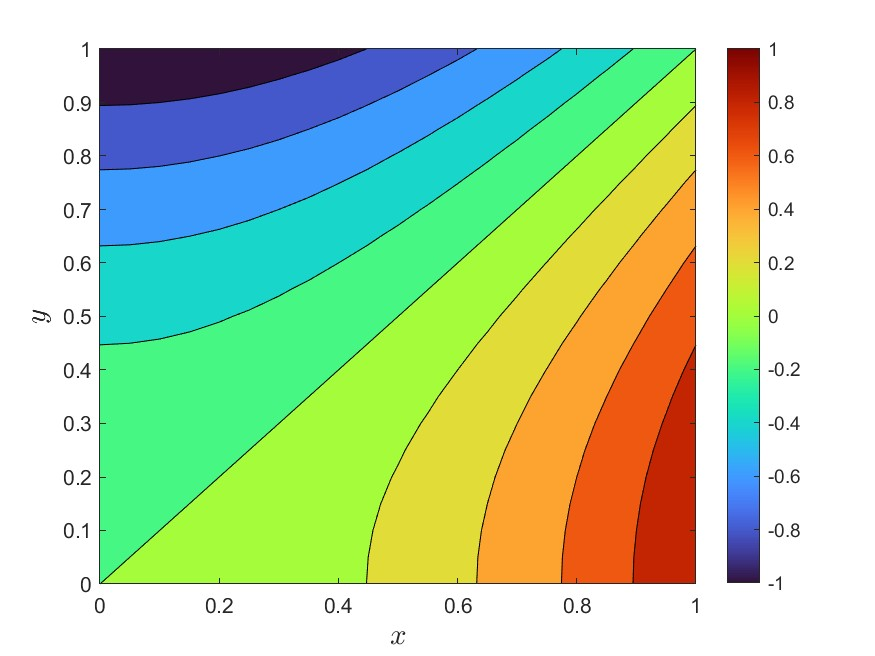
\includegraphics[width=0.55\textwidth]{campo-escalar}
            \caption{Gráfica del campo escalar \(\phi(x, y) = x^{2} - y^{2}\).}
            \label{fig:scalar-field}
        \end{figure}
        
        \item el gradiente del campo escalar.
        
        La gráfica del gradiente del campo escalar \(\grad{{\phi(x, y)}} = (2x, -2y, 0)\) se muestra en la \cref{fig:gradient-scalar-field}.

        \begin{figure}[htb]
            \centering
            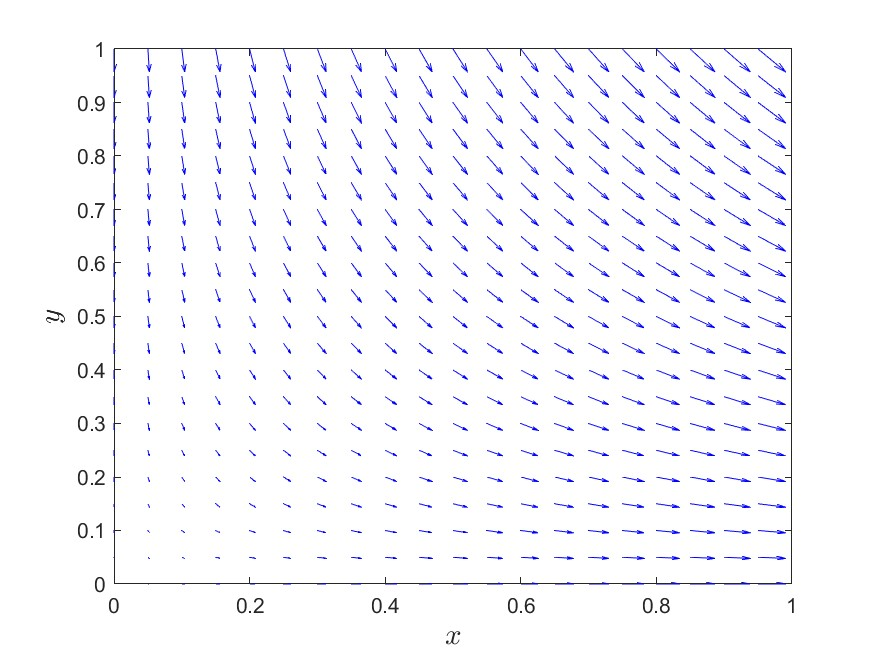
\includegraphics[width=0.6\textwidth]{gradiente-campo-escalar}
            \caption{Gráfica del gradiente del campo escalar \(\grad{{\phi(x, y)}} = (2x, -2y, 0)\).}
            \label{fig:gradient-scalar-field}
        \end{figure}
    \end{enumerate}
\end{document}